%
% stacked.tex
%
\section{Chart::StackedBars}
\name{Chart::StackedBars}
\file{StackedBars.pm}
\requires{Chart::Base, GD, Carp, FileHandle}
\begin{Description} 
\class{StackedBars} is a \fett{subclass} of class \class{Chart::Base}.
The class StackedBars creates a chart with stacked bars.
\end{Description}

\parindent 0pt{\large Example:}

\begin{figure}[h]
	\begin{center}
		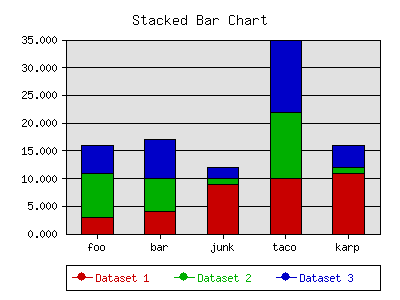
\includegraphics[scale=0.6]{stackedbars.png}
	\end{center}
	\caption{Chart with stacked bars}
	\label{fig:stackedbars}
\end{figure}
\begin{verbatim}
use Chart::StackedBars;

$g = Chart::StackedBars->new;

$g->add_dataset ('foo', 'bar', 'junk', 'taco', 'karp');
$g->add_dataset (3, 4, 9, 10, 11);
$g->add_dataset (8, 6, 1, 12, 1);
$g->add_dataset (5, 7, 2, 13, 4);

$g->set ('title' => 'Stacked Bar Chart');
$g->set('y_grid_lines' => 'true');
$g->set('legend' => 'bottom');

$g->png ("Grafiken/stackedbars.png");
\end{verbatim}

\begin{Constructor} An instance of a stacked bars object can be created with the constructor
\textit{new()}:
\begin{quote}
\fett{\$obj = Chart::StackedBars->new();}\\
\fett{\$obj = Chart::StackedBars->new(\parameter{width}, \parameter{height});}
\end{quote}
If \textit{new()} has no arguments, 
the constructor returns an image with the size 300x400 pixels. 
If \textit{new()} has two arguments \parameter{width} and \parameter{height},
it returns an image with the desired size.
\end{Constructor}

\Methods
All universal valid methods, see page \pageref{methods}
of class \class{Chart::Base}.\\[\parabstand]
%
\Attributes
All universal valid options, see page \pageref{options}. Also available, these special options:
\begin{description}
\item['y\_axes'] Tells chart where to place the y-axis. 
                 Valid values are 'left', 'right' and 'both'. Defaults to 'left'.
\item['spaced\_bars'] Leaves space between the groups of bars at each data point 
                      when set to 'true'.  
                      This just makes it easier to read a bar chart.  Default is 'true'.
\end{description}
